\documentclass[
  stu,
  floatsintext,
  longtable,
  a4paper,
  nolmodern,
  notxfonts,
  notimes,
  colorlinks=true,linkcolor=blue,citecolor=blue,urlcolor=blue]{apa7}

\usepackage{amsmath}
\usepackage{amssymb}



\usepackage[bidi=default]{babel}
\babelprovide[main,import]{spanish}
\StartBabelCommands{spanish}{captions} [unicode, fontenc=TU EU1 EU2, charset=utf8] \SetString{\keywordname}{Palabras
Claves}
\EndBabelCommands


% get rid of language-specific shorthands (see #6817):
\let\LanguageShortHands\languageshorthands
\def\languageshorthands#1{}

\RequirePackage{longtable}
\RequirePackage{threeparttablex}

\makeatletter
\renewcommand{\paragraph}{\@startsection{paragraph}{4}{\parindent}%
	{0\baselineskip \@plus 0.2ex \@minus 0.2ex}%
	{-.5em}%
	{\normalfont\normalsize\bfseries\typesectitle}}

\renewcommand{\subparagraph}[1]{\@startsection{subparagraph}{5}{0.5em}%
	{0\baselineskip \@plus 0.2ex \@minus 0.2ex}%
	{-\z@\relax}%
	{\normalfont\normalsize\bfseries\itshape\hspace{\parindent}{#1}\textit{\addperi}}{\relax}}
\makeatother




\usepackage{longtable, booktabs, multirow, multicol, colortbl, hhline, caption, array, float, xpatch}
\usepackage{subcaption}
\renewcommand\thesubfigure{\Alph{subfigure}}
\setcounter{topnumber}{2}
\setcounter{bottomnumber}{2}
\setcounter{totalnumber}{4}
\renewcommand{\topfraction}{0.85}
\renewcommand{\bottomfraction}{0.85}
\renewcommand{\textfraction}{0.15}
\renewcommand{\floatpagefraction}{0.7}

\usepackage{tcolorbox}
\tcbuselibrary{listings,theorems, breakable, skins}
\usepackage{fontawesome5}

\definecolor{quarto-callout-color}{HTML}{909090}
\definecolor{quarto-callout-note-color}{HTML}{0758E5}
\definecolor{quarto-callout-important-color}{HTML}{CC1914}
\definecolor{quarto-callout-warning-color}{HTML}{EB9113}
\definecolor{quarto-callout-tip-color}{HTML}{00A047}
\definecolor{quarto-callout-caution-color}{HTML}{FC5300}
\definecolor{quarto-callout-color-frame}{HTML}{ACACAC}
\definecolor{quarto-callout-note-color-frame}{HTML}{4582EC}
\definecolor{quarto-callout-important-color-frame}{HTML}{D9534F}
\definecolor{quarto-callout-warning-color-frame}{HTML}{F0AD4E}
\definecolor{quarto-callout-tip-color-frame}{HTML}{02B875}
\definecolor{quarto-callout-caution-color-frame}{HTML}{FD7E14}

%\newlength\Oldarrayrulewidth
%\newlength\Oldtabcolsep


\usepackage{hyperref}




\providecommand{\tightlist}{%
  \setlength{\itemsep}{0pt}\setlength{\parskip}{0pt}}
\usepackage{longtable,booktabs,array}
\usepackage{calc} % for calculating minipage widths
% Correct order of tables after \paragraph or \subparagraph
\usepackage{etoolbox}
\makeatletter
\patchcmd\longtable{\par}{\if@noskipsec\mbox{}\fi\par}{}{}
\makeatother
% Allow footnotes in longtable head/foot
\IfFileExists{footnotehyper.sty}{\usepackage{footnotehyper}}{\usepackage{footnote}}
\makesavenoteenv{longtable}

\usepackage{graphicx}
\makeatletter
\newsavebox\pandoc@box
\newcommand*\pandocbounded[1]{% scales image to fit in text height/width
  \sbox\pandoc@box{#1}%
  \Gscale@div\@tempa{\textheight}{\dimexpr\ht\pandoc@box+\dp\pandoc@box\relax}%
  \Gscale@div\@tempb{\linewidth}{\wd\pandoc@box}%
  \ifdim\@tempb\p@<\@tempa\p@\let\@tempa\@tempb\fi% select the smaller of both
  \ifdim\@tempa\p@<\p@\scalebox{\@tempa}{\usebox\pandoc@box}%
  \else\usebox{\pandoc@box}%
  \fi%
}
% Set default figure placement to htbp
\def\fps@figure{htbp}
\makeatother







\usepackage{newtx}

\defaultfontfeatures{Scale=MatchLowercase}
\defaultfontfeatures[\rmfamily]{Ligatures=TeX,Scale=1}





\title{Proporcionalidad de Magnitudes}


\shorttitle{Proporcionalidad de Magnitudes}


\usepackage{etoolbox}


\course{Matemáticas Aplicadas a la Comunicación}

\ccoppy{\textcopyright~2025}



\author{Edison Achalma}



\affiliation{
{Escuela Profesional de Economía, Universidad Nacional de San Cristóbal
de Huamanga}}




\leftheader{Achalma}

\date{2025-05-20}


\abstract{Este trabajo explora los fundamentos matemáticos de la
proporcionalidad y sus aplicaciones en el campo de las Ciencias de la
Comunicación. Se analizan conceptos clave como razones, proporciones y
magnitudes, junto con sus implementaciones prácticas en estrategias
mediáticas, análisis de audiencias y diseño de mensajes. El estudio
demuestra cómo estas herramientas matemáticas optimizan procesos
comunicacionales en entornos digitales y tradicionales }

\keywords{proporcionalidad, comunicación, matemáticas
aplicadas, análisis de audiencias, estrategias mediáticas}

\authornote{\par{\addORCIDlink{Edison Achalma}{0000-0001-6996-3364}} 
\par{ }
\par{   El autor no tiene conflictos de interés que revelar.  Expreso mi
sincero agradecimiento a todas las personas que contribuyeron directa e
indirectamente a la realización de esta monografía. En especial. A mi
profesor, por su valiosa orientación, correcciones y sugerencias que
permitieron estructurar y mejorar este trabajo. A la institución
educativa y a la Facultad de Ciencias de la Comunicación, por brindar
las herramientas necesarias para mi desarrollo profesional. A los
autores y especialistas cuyas investigaciones sirvieron como base
teórica para este estudio. A mi familia y seres queridos, por su
constante apoyo emocional durante este proceso. Este trabajo es el
resultado de un esfuerzo colectivo, y por ello, mi más profundo
reconocimiento a quienes hicieron posible su culminación.  Los roles de
autor se clasificaron utilizando la taxonomía de roles de colaborador
(CRediT; https://credit.niso.org/) de la siguiente manera:  Edison
Achalma:   conceptualización, redacción}
\par{La correspondencia relativa a este artículo debe dirigirse a Edison
Achalma, Email: \href{mailto:elmer.achalma.09@unsch.edu.pe}{elmer.achalma.09@unsch.edu.pe}}
}

\makeatletter
\let\endoldlt\endlongtable
\def\endlongtable{
\hline
\endoldlt
}
\makeatother

\urlstyle{same}



\makeatletter
\@ifpackageloaded{caption}{}{\usepackage{caption}}
\AtBeginDocument{%
\ifdefined\contentsname
  \renewcommand*\contentsname{Tabla de contenidos}
\else
  \newcommand\contentsname{Tabla de contenidos}
\fi
\ifdefined\listfigurename
  \renewcommand*\listfigurename{Listado de Figuras}
\else
  \newcommand\listfigurename{Listado de Figuras}
\fi
\ifdefined\listtablename
  \renewcommand*\listtablename{Listado de Tablas}
\else
  \newcommand\listtablename{Listado de Tablas}
\fi
\ifdefined\figurename
  \renewcommand*\figurename{Figura}
\else
  \newcommand\figurename{Figura}
\fi
\ifdefined\tablename
  \renewcommand*\tablename{Tabla}
\else
  \newcommand\tablename{Tabla}
\fi
}
\@ifpackageloaded{float}{}{\usepackage{float}}
\floatstyle{ruled}
\@ifundefined{c@chapter}{\newfloat{codelisting}{h}{lop}}{\newfloat{codelisting}{h}{lop}[chapter]}
\floatname{codelisting}{Listado}
\newcommand*\listoflistings{\listof{codelisting}{Listado de Listados}}
\makeatother
\makeatletter
\makeatother
\makeatletter
\@ifpackageloaded{caption}{}{\usepackage{caption}}
\@ifpackageloaded{subcaption}{}{\usepackage{subcaption}}
\makeatother

% From https://tex.stackexchange.com/a/645996/211326
%%% apa7 doesn't want to add appendix section titles in the toc
%%% let's make it do it
\makeatletter
\xpatchcmd{\appendix}
  {\par}
  {\addcontentsline{toc}{section}{\@currentlabelname}\par}
  {}{}
\makeatother

%% Disable longtable counter
%% https://tex.stackexchange.com/a/248395/211326

\usepackage{etoolbox}

\makeatletter
\patchcmd{\LT@caption}
  {\bgroup}
  {\bgroup\global\LTpatch@captiontrue}
  {}{}
\patchcmd{\longtable}
  {\par}
  {\par\global\LTpatch@captionfalse}
  {}{}
\apptocmd{\endlongtable}
  {\ifLTpatch@caption\else\addtocounter{table}{-1}\fi}
  {}{}
\newif\ifLTpatch@caption
\makeatother

\begin{document}

\maketitle

\hypertarget{toc}{}
\tableofcontents
\newpage
\section[Introduction]{Proporcionalidad de Magnitudes}

\setcounter{secnumdepth}{3}

\setlength\LTleft{0pt}


La presente monografía explora el concepto de proporcionalidad y su
relevancia en el campo de las Ciencias de la Comunicación, destacando su
aplicación en estrategias mediáticas, análisis de audiencias y diseño de
mensajes. A través de un enfoque interdisciplinario, este trabajo busca
demostrar cómo las relaciones proporcionales, ya sean aritméticas o
geométricas, permiten optimizar recursos, medir impactos y tomar
decisiones basadas en datos. En un contexto donde la comunicación se
sustenta cada vez más en métricas y algoritmos, comprender estas
herramientas matemáticas se vuelve esencial para profesionales y
académicos del área.

El estudio de la proporcionalidad no es nuevo. Sus raíces se remontan a
la antigua Grecia, donde matemáticos como Euclides y Pitágoras
establecieron sus fundamentos teóricos. Euclides, en su obra
\emph{Elementos}, definió las proporciones como igualdades entre
razones, sentando las bases para su aplicación en geometría y
arquitectura. Más tarde, durante el Renacimiento, artistas como Leonardo
da Vinci emplearon proporciones áureas para crear composiciones visuales
armónicas, mientras que en el siglo XIX, economistas como Léon Walras
las adaptaron para modelar equilibrios de mercado. En el ámbito
comunicacional, su uso sistemático comenzó en el siglo XX con el auge de
la publicidad masiva y la necesidad de medir audiencias mediante ratings
y shares, consolidándose hoy como un pilar en el análisis de big data y
la inteligencia artificial aplicada a medios.

El objetivo principal de esta monografía es analizar cómo la
proporcionalidad, desde sus formas más básicas hasta sus aplicaciones
avanzadas, contribuye a resolver problemas prácticos en la carrera de
ciencias de la comunicación, tales como la distribución de presupuestos
publicitarios, el escalado de piezas gráficas o la interpretación de
estadísticas de engagement.

Este trabajo se desarrolla a lo largo de seis capítulos organizados de
forma progresiva. El Capítulo I se establece los fundamentos teóricos de
razones y proporciones, analizando sus propiedades matemáticas y
clasificaciones. El Capítulo II traslada estos conceptos al plano
práctico, examinando herramientas como reparto proporcional, regla de
tres y porcentajes. El Capítulo III demuestra aplicaciones concretas en
comunicación como análisis de audiencias, diseño gráfico y evaluación de
campañas. Los capítulos finales (IV y V) presentan las conclusiones,
recomendaciones y referencias bibliográficas.

\section{Capítulo I Marco Teórico y
Conceptual}\label{capuxedtulo-i-marco-teuxf3rico-y-conceptual}

\subsection{Razón}\label{razuxf3n}

La razón es una relación entre dos magnitudes del mismo tipo, expresada
generalmente como una comparación de cantidades.

\subsubsection{Razón Aritmética}\label{razuxf3n-aritmuxe9tica}

La razón aritmética se define como la diferencia entre dos magnitudes,
expresada como una relación que compara su valor absoluto.

\textbf{Fórmula de razón aritmética}

\[
r = a_{n} - a_{n-1}
\]

Donde:

\begin{itemize}
\item
  \(r\) es la razón aritmética.
\item
  \(a_{n}\) es el término en la posición \(n\).
\item
  \(a_{n-1}\) es el término en la posición \(n-1\).
\item
  \(n\) es la posición del término.
\item
  \(a_{1}\) es el primer término.
\end{itemize}

\subsubsection{Razón Geométrica}\label{razuxf3n-geomuxe9trica}

La razón geométrica se define como el cociente entre dos magnitudes,
expresando cuántas veces una contiene a la otra. Daniele Barbaro, en su
comentario sobre \emph{De Architectura} de Vitruvio, define la razón
geométrica como ``la relación determinada, respeto o comparación entre
dos cantidades comprendidas dentro del mismo género, como es el caso de
dos números, o dos sólidos, o dos lugares, dos tiempos, dos líneas, dos
planos'' (Barbaro, 1567, en Williams, 2019, p.~176).

\textbf{Fórmula de razón geométrica}

\[
r = \frac{a_{n}}{a_{n-1}}
\]

Donde:

\begin{itemize}
\item
  \(r\) es la razón geométrica.
\item
  \(a_{n}\) es el término en la posición \(n\).
\item
  \(a_{n-1}\) es el término en la posición \(n-1\).
\item
  \(n\) es la posición del término.
\item
  \(a_{1}\) es el primer término.
\end{itemize}

\subsection{Propociones}\label{propociones}

\subsubsection{Proporción Aritmética}\label{proporciuxf3n-aritmuxe9tica}

\paragraph{Concepto y Definición.}\label{concepto-y-definiciuxf3n}

Una proporción aritmética es una relación de igualdad entre las
diferencias de dos pares de magnitudes, donde la diferencia entre los
términos de un par es igual a la diferencia entre los términos del otro
par. Según Rico (2008), ``una proporción aritmética se establece cuando
tres cantidades están dispuestas de manera que la diferencia entre la
segunda y la primera es igual a la diferencia entre la tercera y la
segunda'' (p.~62).

\paragraph{Representación
Matemática.}\label{representaciuxf3n-matemuxe1tica}

En una proporción aritmética, se comparan dos pares de magnitudes ( a, b
) y ( c, d ). La relación se expresa como:

\[
a - b = c - d
\]

donde:

\begin{itemize}
\item
  \(a-c\) son los términos extremos
\item
  \(b-d\) son los términos medios
\end{itemize}

\paragraph{Ejemplo.}\label{ejemplo}

Supóngase que se analizan las menciones de un concepto comunicacional en
tres días consecutivos: lunes (20 menciones), martes (30 menciones), y
miércoles (40 menciones). Estos valores forman una proporción aritmética
porque:

\[
30 - 20 = 10 \quad \text{y} \quad 40 - 30 = 10
\]

\subsubsection{Proporción Geométrica}\label{proporciuxf3n-geomuxe9trica}

\paragraph{Concepto y Definición.}\label{concepto-y-definiciuxf3n-1}

Una proporción geométrica es una relación de igualdad entre los
cocientes de dos pares de magnitudes, donde el cociente entre los
términos de un par es igual al cociente entre los términos del otro par.

Tal como lo define D'Amore (2005), ``tres números están en proporción
geométrica cuando el segundo es media proporcional entre el primero y el
tercero, es decir, cuando el cuadrado del segundo es igual al producto
del primero por el tercero'' (p.~91).

\paragraph{Representación
Matemática.}\label{representaciuxf3n-matemuxe1tica-1}

En una proporción geométrica, se comparan dos pares de magnitudes ( a, b
) y ( c, d ). La relación se expresa como:

\[
\frac{a}{b} = \frac{c}{d}
\]

Donde: - \(a\) y \(c\) son los términos extremos - \(b\) y \(d\) son los
términos medios

Equivalentemente, el producto de los términos extremos iguala el
producto de los términos medios:

\[
a \cdot d = b \cdot c
\]

\paragraph{Ejemplo.}\label{ejemplo-1}

En una campaña publicitaria, se comparan los alcances en dos
plataformas. Si la plataforma A genera 40,000 impresiones con un
presupuesto de 8,000 dólares, y la plataforma B genera 20,000
impresiones con 4,000 dólares, se verifica la proporción geométrica:

\[
\frac{40000}{8000} = \frac{20000}{4000}
\]

\[
5 = 5
\]

Alternativamente, usando los términos medios y extremos:

\[
40000 \cdot 4000 = 8000 \cdot 20000
\]

\[
160,000,000 = 160,000,000
\]

La igualdad nos indica que los alcances y presupuestos forman una
proporción geométrica, útil para evaluar la eficiencia relativa de las
plataformas.

\subsubsection{Propiedades de la Proporción
Geométrica}\label{propiedades-de-la-proporciuxf3n-geomuxe9trica}

Sea la proporción \(\frac{a}{b} = \frac{c}{d}\)

\begin{itemize}
\item
  \(\frac{a+b}{a} = \frac{c+d}{c}\)
\item
  \(\frac{a-b}{b} = \frac{c-d}{d}.\)
\item
  \(\frac{a+b}{a-b} = \frac{c+d}{c-d}\)
\item
  \(\frac{a^n}{b^n} = \frac{c^n}{d^n} ; \quad n \in \mathbb{Q}\)
\item
  \(\frac{a-c}{b-d} = \frac{a}{b} = \frac{c}{d}\)
\end{itemize}

\subsubsection{Series de Razones Geométricas
Equivalentes}\label{series-de-razones-geomuxe9tricas-equivalentes}

\paragraph{Concepto y Definición.}\label{concepto-y-definiciuxf3n-2}

Una serie de razones geométricas equivalentes es una secuencia de
proporciones geométricas que comparten la misma razón constante,
permitiendo modelar crecimientos o disminuciones proporcionales.

Según Gómez (2011), ``una serie geométrica se define como una sucesión
de razones equivalentes en la que cada razón se obtiene multiplicando la
anterior por un mismo valor constante denominado razón común'' (p.~135).
Esta definición implica que en una serie como
\(\frac{a_1}{c_1}, \frac{a_2}{c_2}, \frac{a_3}{c_3}, \dots\), todas las
fracciones son equivalentes y se cumple que:

\[
\frac{a_1}{c_1} = \frac{a_2}{c_2} = \frac{a_3}{c_3} = \cdots = r
\]

Donde:

\begin{itemize}
\item
  \(a_1, a_2, a_3, \dots\) son los antecedentes.
\item
  \(c_1, c_2, c_3, \dots\) son los consecuentes.
\item
  \(r\) es la razón constante.
\end{itemize}

La fórmula general para una serie geométrica es:

\[
a_n = a_1 \cdot r^{n-1}
\]

Donde:

\begin{itemize}
\item
  \(a_n\) es el \(n\)-ésimo término
\item
  \(a_1\) es el primer término
\item
  \(r\) es la razón constante
\item
  \(n\) es la posición del término.
\end{itemize}

\textbf{Ejemplo}

En una campaña viral, el número de compartidos de un video en una red
social crece según una serie geométrica. En el primer día, el video
tiene 1000 compartidos (\(a_1 = 1000\)). Cada día, el número de
compartidos se multiplica por una razón constante (\(r = 2\)). Para el
cuarto día (\(n = 4\)), calculamos el número de compartidos:

\[
a_4 = a_1 \cdot r^{4-1} = 1000 \cdot 2^3 = 1000 \cdot 8 = 8000
\]

Verificamos la proporción geométrica para los días 1 y 2
(\(a_1 = 1000\), \(a_2 = 2000\)) y días 3 y 4 (\(a_3 = 4000\),
\(a_4 = 8000\)):

\[
\frac{a_2}{a_1} = \frac{2000}{1000} = 2
\]

\[
\frac{a_4}{a_3} = \frac{8000}{4000} = 2
\]

\[
\frac{a_2}{a_1} = \frac{a_4}{a_3} \implies 2 = 2
\]

\paragraph{Propiedades.}\label{propiedades}

\begin{enumerate}
\def\labelenumi{\arabic{enumi}.}
\item
  \(\frac{a_1+a_2+a_3 + ... + a_n }{c_1+c_2+c_3 + ... + c_n} = k\),
  Textualmente,
  \(\frac{\text{la suma de los antecedentes}  }{\text{Suma de consecuentes}} = \text{Razón}\)
\item
  \(\frac{a_1*a_2*a_3 * ... * a_n }{c_1*c_2*c_3 * ... * c_n} = k^n\),
  Textualmente,
  \(\frac{\text{Producto de los antecedentes}  }{\text{Producto de consecuentes}} = \text{Razón}^n\)
\end{enumerate}

Donde \(n\) es el número de términos de la serie.

\subsection{Tipos y Clasificaciones de
Proporcionalidad}\label{tipos-y-clasificaciones-de-proporcionalidad}

\subsubsection{Proporcionalidad
Discreta}\label{proporcionalidad-discreta}

\paragraph{Aritmética.}\label{aritmuxe9tica}

La proporcionalidad discreta aritmética establece una relación entre
cuatro magnitudes donde la diferencia entre dos términos es igual a la
diferencia entre otros dos. La relación se expresa como:

\[
a - b = c - d
\]

Donde:

\begin{itemize}
\tightlist
\item
  \(d\) es la cuarta diferencial de \(a\), \(b\) y \(c\).
\end{itemize}

\textbf{Ejemplo:} Una empresa distribuye anuncios en dos plataformas de
redes sociales, asignando 20 espacios el primer día en Facebook
(\(a = 20\)) y 15 en Instagram (\(b = 15\)). El segundo día, asigna 30
espacios en Facebook (\(c = 30\)) y desea calcular los espacios en
Instagram (\(d\)) para mantener la proporcionalidad aritmética discreta.
Usamos la fórmula:

\[
a - b = c - d
\]

\[
20 - 15 = 30 - d
\]

\[
5 = 30 - d
\]

\[
5 = 30 - d \implies d = 30 - 5 = 25
\]

Por lo tanto, se asignan 25 espacios en Instagram el segundo día.
Verificamos:

\[
20 - 15 = 5
\]

\[
30 - 25 = 5
\]

Vemos que la proporcionalidad aritmética discreta asegura una
distribución equitativa de recursos publicitarios.

\paragraph{Geométrica.}\label{geomuxe9trica}

La proporcionalidad discreta geométrica describe una relación entre
cuatro magnitudes donde el cociente entre dos términos es igual al
cociente entre otros dos. La relación se expresa como:

\[
\frac{a}{b} = \frac{c}{d}
\]

Donde:

\begin{itemize}
\tightlist
\item
  \(d\) es la cuarta proporcional de \(a\), \(b\) y \(c\).
\end{itemize}

\textbf{Ejemplo:} Una campaña digital genera 600 interacciones con un
presupuesto de 200 \((a = 600, b = 200)\). Para un segundo presupuesto
de 500 \((d = 500)\), se desea calcular las interacciones esperadas
(\(c\)) manteniendo la proporcionalidad geométrica discreta:

\[
\frac{a}{b} = \frac{c}{d}
\]

\[
\frac{600}{200} = \frac{c}{500}
\]

\[
3 = \frac{c}{500} \implies c = 3 \cdot 500 = 1500
\]

Se esperan 1500 interacciones. Verificamos:

\[
\frac{600}{200} = 3
\]

\[
\frac{1500}{500} = 3
\]

Vemos cómo la proporcionalidad geométrica discreta modela el crecimiento
proporcional de interacciones según el presupuesto.

\subsubsection{Proporcionalidad
Continua}\label{proporcionalidad-continua}

\paragraph{Aritmética.}\label{aritmuxe9tica-1}

La proporcionalidad continua aritmética describe una relación entre tres
magnitudes. La relación se expresa como:

\[
a - b = b - c
\]

Donde: - \(c\) es la tercera diferencial de \(a\) y \(b\), y \(b\) es la
media diferencial de \(a\) y \(c\).

\textbf{Ejemplo:} Una emisora de radio asigna tiempos de publicidad (en
minutos) en tres programas consecutivos. Si el primer programa tiene 10
minutos (\(a = 10\)), el segundo 7 minutos (\(b = 7\)), se calcula el
tiempo del tercer programa (\(c\)):

\[
a - b = b - c
\]

\[
10 - 7 = 7 - c
\]

\[
3 = 7 - c \implies c = 7 - 3 = 4
\]

El tercer programa tiene 4 minutos. Verificamos:

\[
10 - 7 = 3
\]

\[
7 - 4 = 3
\]

Vemos cómo la proporcionalidad aritmética continua modela la asignación
uniforme de tiempos en medios.

\paragraph{Geométrica.}\label{geomuxe9trica-1}

La proporcionalidad continua geométrica describe una relación entre tres
magnitudes. La relación se expresa as:

\[
\frac{a}{b} = \frac{b}{c}
\]

Donde:

\begin{itemize}
\tightlist
\item
  \(c\) es la tercera proporcional de \(a\) y \(b\), y \(b\) es la media
  proporcional de \(a\) y \(c\), implicando:
\end{itemize}

\[
b^2 = a \cdot c
\]

\textbf{Ejemplo:} En una campaña viral, el número de visualizaciones
diarias de un video es 1000 el primer día (\(a = 1000\)), 2000 el
segundo día (\(b = 2000\)). Calculamos las visualizaciones del tercer
día (\(c\)):

\[
\frac{a}{b} = \frac{b}{c}
\]

\[
\frac{1000}{2000} = \frac{2000}{c}
\]

\[
\frac{1}{2} = \frac{2000}{c} \implies c = 2000 \cdot 2 = 4000
\]

El tercer día tiene 4000 visualizaciones. Verificamos:

\[
b^2 = a \cdot c
\]

\[
2000^2 = 1000 \cdot 4000
\]

\[
4,000,000 = 4,000,000
2000^2 = 1000 \cdot 4000
\]

\[
4,000,000 = 4,000,000
\]

\subsection{Magnitudes Proporcionales}\label{magnitudes-proporcionales}

\subsubsection{Definición y Tipos}\label{definiciuxf3n-y-tipos}

\paragraph{Magnitudes Directamente
Proporcionales.}\label{magnitudes-directamente-proporcionales}

Una magnitud directamente proporcional se define como una relación entre
dos cantidades donde el aumento de una implica un incremento
proporcional en la otra, manteniendo una constante fija. En el ámbito
publicitario, esto se observa, por ejemplo, en la relación entre el
presupuesto destinado a una campaña y el número de impresiones
generadas. Matemáticamente, si \(x\) representa el presupuesto (en miles
de dólares) y \(y\) el número de impresiones (en miles), la relación se
expresa como:

\[
\frac{y}{x} = k
\]

\[
y = kx
\]

Donde:

\begin{itemize}
\tightlist
\item
  \(y\) es la magnitud dependiente (número de impresiones).
\item
  \(x\) es la magnitud independiente (presupuesto).
\item
  \(k\) es la constante de proporcionalidad.
\end{itemize}

\textbf{Ejemplo}: Relación entre presupuesto y alcance de impresiones

Supongamos una campaña digital con los siguientes datos:

\begin{table}

{\caption{{Relación entre Presupuesto e
Impresiones}{\label{tbl-mytable2}}}}

\begin{longtable}[]{@{}ll@{}}
\toprule\noalign{}
Presupuesto (\(x\), en miles de dólares) & Impresiones (\(y\), en
miles) \\
\midrule\noalign{}
\endhead
\bottomrule\noalign{}
\endlastfoot
1 & 10 \\
2 & 20 \\
3 & 30 \\
4 & 40 \\
\end{longtable}

{\noindent \emph{Note.} Elaboración propia}

\end{table}

Vemos que el presupuesto y el número de impresiones son directamente
proporcionales.

Luego:

\[
\frac{valor de presupuesto}{valor de impresiones} = \frac{1}{10} = \frac{2}{20} = \frac{3}{30} = \frac{4}{40} = Constante
\]

La constante de proporcionalidad es:

\[
k = \frac{y}{x} = \frac{10}{1} = 10
\]

\paragraph{Gráficamente.}\label{gruxe1ficamente}

La gráfica de una función de proporcionalidad directa es una recta que
pasa por el origen, con pendiente igual a la constante \(k\).

La ecuación de la recta es:

\[
y = k \cdot x
\]

Donde: \(k\) es la constante de proporcionalidad.

\pandocbounded{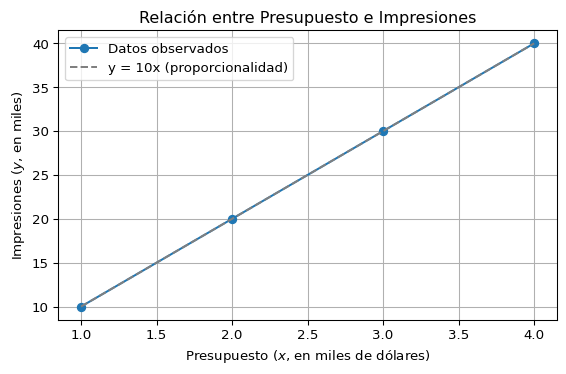
\includegraphics[keepaspectratio]{index_files/figure-pdf/cell-2-output-1.png}}

\paragraph{En general.}\label{en-general}

\begin{table}

{\caption{{Magnitudes directamente
proporcionales}{\label{tbl-mytable2}}}}

\begin{longtable}[]{@{}ll@{}}
\toprule\noalign{}
\(x\) & \(y\) \\
\midrule\noalign{}
\endhead
\bottomrule\noalign{}
\endlastfoot
\(x_1\) & \(kx_1\) \\
\(x_2\) & \(kx_2\) \\
\(x_3\) & \(kx_3\) \\
\end{longtable}

{\noindent \emph{Note.} Elaboración propia}

\end{table}

donde se cumple que:

\[
\frac{y_1}{x_1} = \frac{y_2}{x_2} = \frac{y_3}{x_3} = k
\]

Lo que denotamos:

\[
\frac{y_i}{x_i} = k
\]

donde k es la constante de proporcionalidad directa. \(1 <= i < n\) ; i
pertenece a \(\mathbb{Z}\)

\paragraph{Funcion de proporcionalidad
directa.}\label{funcion-de-proporcionalidad-directa}

Se expresa mediante la función lineal homogénea:

\[
f(x) = kx
\]

donde \(f(x)\) representa la magnitud dependiente.

\paragraph{Ejemplo.}\label{ejemplo-2}

Si una agencia de medios cobra \$500 por cada 1,000 impresiones
generadas, el número de impresiones por \$3,000 se calcula como:

\[
y = 1000 \cdot \frac{3000}{500} = 6000
\]

\paragraph{Magnitudes Inversamente
Proporcionales.}\label{magnitudes-inversamente-proporcionales}

Las magnitudes inversamente proporcionales son aquellas en las que el
incremento de una magnitud provoca una disminución proporcional en la
otra, manteniendo su producto constante. En la planificación de medios,
esto aplica a la relación entre el tiempo de exposición de un anuncio y
la frecuencia de publicación necesaria para un impacto constante. Según
Arican y Kiymaz (2022), ``una forma de proporción en la que un valor
aumenta mientras que el otro disminuye, y hay una relación constante
entre ellos'' (p.~6). Matemáticamente, si \(x\) es el tiempo de
exposición (en segundos) y \(y\) la frecuencia de publicación (en
publicaciones por día), la relación se expresa como:

\[
\frac{y}{x} = k
\]

\[
x \cdot y = k
\]

Donde:

\begin{itemize}
\tightlist
\item
  \(k\) es la constante de proporcionalidad inversa.
\end{itemize}

\begin{table}

{\caption{{Relación entre tiempo de exposición y
frecuencia}{\label{tbl-mytable2}}}}

\begin{longtable}[]{@{}
  >{\raggedright\arraybackslash}p{(\linewidth - 2\tabcolsep) * \real{0.5065}}
  >{\raggedright\arraybackslash}p{(\linewidth - 2\tabcolsep) * \real{0.4935}}@{}}
\toprule\noalign{}
\begin{minipage}[b]{\linewidth}\raggedright
Tiempo de exposición (\(x\), en segundos)
\end{minipage} & \begin{minipage}[b]{\linewidth}\raggedright
Frecuencia (\(y\), en publicaciones/día)
\end{minipage} \\
\midrule\noalign{}
\endhead
\bottomrule\noalign{}
\endlastfoot
5 & 20 \\
10 & 10 \\
20 & 5 \\
40 & 2.5 \\
\end{longtable}

{\noindent \emph{Note.} Elaboración propia}

\end{table}

Vemos que el tiempo de exposición y la frecuencia son inversamente
proporcionales. Luego:

\[
(valor de tiempo)*(valor de frecuencia) = (5)*(20) = (10)*(10) = (20)*(5) = (40)*(2.5) = Constante
\]

La constante de proporcionalidad inversa es:

\[
x \cdot y = 5 \cdot 20 = 100
\]

\paragraph{Gráficamente.}\label{gruxe1ficamente-1}

La gráfica de una función inversamente proporcional es una hipérbola con
asíntotas en los ejes.

\pandocbounded{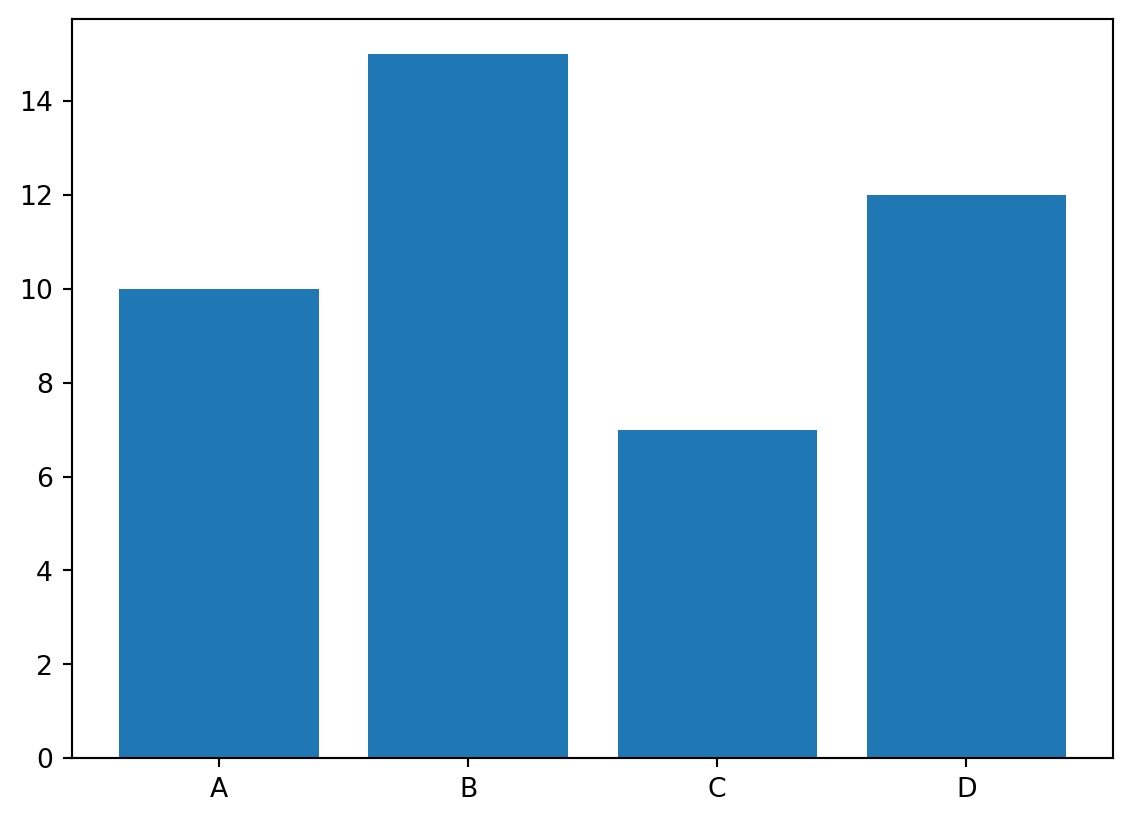
\includegraphics[keepaspectratio]{index_files/figure-pdf/cell-3-output-1.png}}

La gráfica muestra cómo a medida que aumenta el tiempo de exposición, la
frecuencia de publicaciones disminuye, manteniendo una relación inversa.

\paragraph{En general.}\label{en-general-1}

\begin{table}

{\caption{{Magnitudes inversamente
proporcionales}{\label{tbl-mytable2}}}}

\begin{longtable}[]{@{}ll@{}}
\toprule\noalign{}
\(x\) & \(y\) \\
\midrule\noalign{}
\endhead
\bottomrule\noalign{}
\endlastfoot
\(x_1\) & \(\frac{k}{x_1}\) \\
\(x_2\) & \(\frac{k}{x_2}\) \\
\(x_3\) & \(\frac{k}{x_3}\) \\
\end{longtable}

{\noindent \emph{Note.} Elaboración propia}

\end{table}

donde se cumple que:

\[
x_1 \cdot y_1 = x_2 \cdot y_2 = x_3 \cdot y_3 = ... = X_n \cdot Y_n = k
\]

Lo que denotamos:

\[
\frac{y_i}{x_i} = k
\]

donde k es la constante de proporcionalidad inversa. \(1 <= i < n\) ; i
pertenece a \(\mathbb{Z}\)

\paragraph{Funcion de proporcionalidad
inversa.}\label{funcion-de-proporcionalidad-inversa}

La función de proporcionalidad inversa se expresa como:

\[
f(x) * x = k
\]

donde \(f(x)\) representa la magnitud dependiente.

\paragraph{Ejemplo.}\label{ejemplo-3}

Si se busca mantener constante un nivel de impacto mediático de 100
unidades por día, y el tiempo de exposición baja a 4 segundos por
anuncio, entonces la frecuencia óptima es:

\[
y = \frac{100}{4} = 25\ \text{publicaciones/día}
\]

\subsubsection{Propiedades}\label{propiedades-1}

Sean las magnitudes \(x\) e \(y\), entonces:

\begin{enumerate}
\item si $ x \text{ DP } y \Rightarrow y \text{ DP } x $
    \item $ x \text{ IP } y \Rightarrow y \text{ IP } x$
\item $ x \text{ IP } y \Leftrightarrow x \text{ DP } \left( \frac{1}{y} \right) $
\item $ x \text{ DP } y \Leftrightarrow x \text{ IP } \left( \frac{1}{y} \right) $
\item Si $ n \in \mathbb{Q} $, entonces:
\begin{itemize}
\item $ x \text{ DP } y \Leftrightarrow x^n \text{ DP } y^n $
\item $ x \text{ IP } y \Leftrightarrow x^n \text{ IP } y^n $
\end{itemize}
\end{enumerate}

\section{Capítulo II Aplicaciones de las Magnitudes
Proporcionales}\label{capuxedtulo-ii-aplicaciones-de-las-magnitudes-proporcionales}

\subsection{Reparto Proporcional}\label{reparto-proporcional}

\subsubsection{Concepto y Tipos}\label{concepto-y-tipos}

El reparto proporcional es un procedimiento matemático que distribuye
una cantidad total entre varias partes según una proporción determinada,
ya sea directa o inversa, en función de una variable de referencia. Este
concepto se divide en dos tipos principales: reparto directo e inverso.

El reparto directo consiste en distribuir una cantidad total entre
varias partes en proporción directa a una magnitud de referencia, de
modo que a mayor valor de la magnitud, mayor es la cantidad asignada. La
fórmula para el reparto directo es:

\[
x_i = \frac{a_i}{\sum a_i} \cdot T
\]

donde \(x_i\) es la cantidad asignada a la parte \(i\), \(a_i\) es la
magnitud de referencia para la parte \(i\), \(\sum a_i\) es la suma de
todas las magnitudes de referencia, y \(T\) es la cantidad total a
repartir.

\textbf{Ejemplo:} Una empresa de publicidad desea distribuir un
presupuesto de \$10,000 entre tres plataformas digitales según el número
de seguidores: Plataforma A (20,000 seguidores, \(a_1 = 20,000\)),
Plataforma B (30,000 seguidores, \(a_2 = 30,000\)), y Plataforma C
(50,000 seguidores, \(a_3 = 50,000\)).

Solución

Repartir proporcionalmente el presupuesto de \$10,000 entre las tres
plataformas.

La suma de seguidores es:

\[
\sum a_i = 20,000 + 30,000 + 50,000 = 100,000
\]

Calculamos el reparto para cada plataforma:

\[
x_1 = \frac{20,000}{100,000} \cdot 10,000 = 2,000
\]

\[
x_2 = \frac{30,000}{100,000} \cdot 10,000 = 3,000
\]

\[
x_3 = \frac{50,000}{100,000} \cdot 10,000 = 5,000
\]

Verificamos: \(2,000 + 3,000 + 5,000 = 10,000\).

\subsection{Regla de Tres}\label{regla-de-tres}

\subsubsection{Regla de Tres Simple}\label{regla-de-tres-simple}

La regla de tres simple es un procedimiento matemático que permite
encontrar un cuarto valor desconocido a partir de tres valores
conocidos, en relaciones de proporcionalidad directa o inversa entre dos
magnitudes. por ejemplo, para estimar el alcance de un mensaje en redes
sociales si se conoce su comportamiento en un grupo reducido. Por
ejemplo:

\begin{quote}
Si una campaña obtuvo 1,200 visualizaciones al ser publicada en 3
páginas, ¿cuántas visualizaciones tendría si se publica en 7 páginas del
mismo alcance?
\end{quote}

Dado que la relación es directamente proporcional:

\[
\frac{1200}{3} = \frac{x}{7} \Rightarrow x = \frac{1200 \times 7}{3} = 2800
\]

Por lo tanto, al publicarse en 7 páginas, se estiman \textbf{2,800
visualizaciones}.

En caso de proporcionalidad inversa ---por ejemplo, tiempo de edición y
cantidad de editores trabajando simultáneamente---, el planteamiento
varía:

\begin{quote}
Si 4 editores terminan de transcribir una entrevista en 6 horas, ¿cuánto
tiempo tomaría si trabajan 8 editores?
\end{quote}

Como es una relación inversa:

\[
4 \times 6 = 8 \times x \Rightarrow x = \frac{4 \times 6}{8} = 3
\]

El trabajo se completaría en \textbf{3 horas}.

\subsubsection{Regla de Tres Compuesta}\label{regla-de-tres-compuesta}

La regla de tres compuesta se utiliza cuando intervienen más de dos
magnitudes relacionadas proporcionalmente. Su aplicación implica
analizar el tipo de proporcionalidad (directa o inversa) que cada una de
las magnitudes guarda con respecto a la incógnita.

Un ejemplo aplicado a la planificación de medios es el siguiente:

\begin{quote}
Si 3 editores subtitulan 10 videos en 5 días, ¿cuántos días necesitarán
6 editores para subtitular 20 videos del mismo tipo?
\end{quote}

Se organiza la información:

\begin{longtable}[]{@{}llll@{}}
\toprule\noalign{}
Magnitud & Valor 1 & Valor 2 & Relación con días \\
\midrule\noalign{}
\endhead
\bottomrule\noalign{}
\endlastfoot
Editores & 3 & 6 & Inversa \\
Videos & 10 & 20 & Directa \\
Días (incógnita) & 5 & x & --- \\
\end{longtable}

Aplicando la regla de tres compuesta:

\[
x = 5 \times \frac{3}{6} \times \frac{20}{10} = 5 \times 0.5 \times 2 = 5
\]

El resultado es \textbf{5 días}, ya que el aumento en el número de
editores compensa el aumento en la carga de trabajo.

\subsection{Porcentajes}\label{porcentajes}

\subsubsection{Concepto de Porcentaje como Forma de
Proporcionalidad}\label{concepto-de-porcentaje-como-forma-de-proporcionalidad}

El porcentaje es una expresión matemática que representa una relación
proporcional entre una parte y un todo, tomando como base el número
cien. Es una forma de expresar razones o fracciones en términos de ``por
cada cien'', facilitando la comparación y análisis de datos,
especialmente en contextos comunicacionales como encuestas, métricas de
audiencia o análisis de participación.

Por ejemplo, al evaluar la efectividad de una campaña, se puede indicar
que el \textbf{60\,\% del público objetivo} fue alcanzado, lo cual
representa una forma clara y estandarizada de presentar la proporción de
impacto.

\subsubsection{Cálculo de Porcentajes}\label{cuxe1lculo-de-porcentajes}

El cálculo de porcentajes se realiza mediante la siguiente fórmula:

\[
\text{Porcentaje} = \left( \frac{\text{Parte}}{\text{Todo}} \right) \times 100
\]

También puede despejarse para encontrar la parte o el todo:

\begin{itemize}
\item
  Para hallar la parte:

  \[
  \text{Parte} = \left( \frac{\text{Porcentaje} \times \text{Todo}}{100} \right)
  \]
\item
  Para hallar el todo: \[
  \text{Todo} = \left( \frac{\text{Parte} \times 100}{\text{Porcentaje}} \right)
  \]
\end{itemize}

\textbf{Ejemplo}:\\
Si se sabe que \textbf{el 75\,\% de los encuestados} recuerda una
campaña de concientización, y el número total de encuestados fue de 400
personas:

\[
\text{Parte} = \frac{75 \times 400}{100} = 300
\]

\textbf{300 personas} recordaron la campaña.

\paragraph{Aumentos Porcentuales.}\label{aumentos-porcentuales}

Un aumento porcentual indica en cuánto se ha incrementado una cantidad
respecto a su valor original, expresado como porcentaje.

La fórmula para calcular el nuevo valor con aumento porcentual es:

\[
\text{Nuevo valor} = \text{Valor inicial} \times \left(1 + \frac{\text{Porcentaje de aumento}}{100} \right)
\]

\textbf{Ejemplo}:\\
Una emisora radial tenía 1,200 oyentes mensuales y se registra un
aumento del 25\,\% en su audiencia tras una campaña de difusión:

\[
\text{Nuevo valor} = 1200 \times \left(1 + \frac{25}{100}\right) = 1200 \times 1.25 = 1500
\]

La audiencia aumentó a \textbf{1,500 oyentes}.

\paragraph{Descuentos Porcentuales.}\label{descuentos-porcentuales}

El descuento porcentual representa una disminución relativa respecto a
un valor original. Es útil, por ejemplo, en el análisis de pérdidas de
audiencia o reducción de presupuesto en campañas.

La fórmula para calcular el nuevo valor tras un descuento es:

\[
\text{Nuevo valor} = \text{Valor inicial} \times \left(1 - \frac{\text{Porcentaje de descuento}}{100} \right)
\]

\textbf{Ejemplo}:\\
Si un medio digital reduce su presupuesto mensual para publicidad de S/
3,000 a un 20\,\% menos:

\[
\text{Nuevo valor} = 3000 \times (1 - \frac{20}{100}) = 3000 \times 0.8 = 2400
\]

El nuevo presupuesto es de \textbf{S/ 2,400}.

\section{Capítulo III Ejemplos Aplicados y Estudios de
Caso}\label{capuxedtulo-iii-ejemplos-aplicados-y-estudios-de-caso}

\subsection{Aplicaciones en Ciencias de la
Comunicación}\label{aplicaciones-en-ciencias-de-la-comunicaciuxf3n}

\subsubsection{Análisis de Audiencias}\label{anuxe1lisis-de-audiencias}

\paragraph{Ratings y Share.}\label{ratings-y-share}

En el análisis de audiencias, dos indicadores fundamentales son el
\textbf{rating} y el \textbf{share}, ambos expresados como porcentajes.
El rating representa la proporción del total de la población que
visualiza un contenido, mientras que el share indica la proporción sobre
el total de personas que están consumiendo algún medio en un momento
dado.

Como señalan Martínez y Piñuel (2011), ``el rating es el cociente entre
el número de individuos que ven un programa y el universo total
considerado, mientras que el share es el porcentaje que representa esa
audiencia respecto al total de los que están utilizando el medio en ese
instante'' (p.~147).

Por ejemplo, si 1,800 personas ven un noticiero y el universo total es
de 10,000 individuos:

\[
\text{Rating} = \left( \frac{1800}{10000} \right) \times 100 = 18\%
\]

Si, en ese mismo momento, 3,000 personas están viendo televisión:

\[
\text{Share} = \left( \frac{1800}{3000} \right) \times 100 = 60\%
\]

\paragraph{Proporcionalidad en la Distribución de Medios o
Mensajes.}\label{proporcionalidad-en-la-distribuciuxf3n-de-medios-o-mensajes}

La proporcionalidad permite determinar cómo se deben distribuir mensajes
o materiales en función del alcance previsto por zona, medio o segmento
demográfico. Esta herramienta es crucial para maximizar el impacto de la
estrategia comunicacional.

Ejemplo aplicado: Si una campaña debe llegar a 12,000 personas en tres
ciudades con poblaciones proporcionales de 2:3:5, la distribución de
materiales será:

\begin{itemize}
\tightlist
\item
  Total de partes: \(2 + 3 + 5 = 10\)
\item
  Ciudad A: \(\frac{2}{10} \times 12000 = 2400\)
\item
  Ciudad B: \(\frac{3}{10} \times 12000 = 3600\)
\item
  Ciudad C: \(\frac{5}{10} \times 12000 = 6000\)
\end{itemize}

Esto garantiza una distribución equitativa según el tamaño del público
objetivo.

\subsubsection{Escalas en el Diseño Gráfico o
Audiovisual}\label{escalas-en-el-diseuxf1o-gruxe1fico-o-audiovisual}

El uso de escalas proporcionales es esencial en la producción visual. En
diseño gráfico y audiovisual, se debe mantener la proporcionalidad de
los elementos al redimensionarlos para evitar distorsiones y asegurar
coherencia visual.

Según Rodríguez Morales (2012), ``la escala gráfica implica una
transformación proporcional de las dimensiones originales, conservando
la relación entre ancho y alto, lo cual es crucial para la legibilidad y
la armonía visual'' (p.~59).

\textbf{Ejemplo aplicado}:\\
Si un logotipo mide 12\,cm de ancho por 8\,cm de alto, y se desea
escalarlo a 18\,cm de ancho, la altura debe calcularse usando proporción
directa:

\[
\frac{12}{8} = \frac{18}{x} \Rightarrow x = \frac{18 \times 8}{12} = 12\,\text{cm}
\]

La nueva dimensión será de 18\,cm × 12\,cm, conservando su forma
original.

\subsubsection{Análisis de Frecuencia de Aparición de Palabras en
Textos}\label{anuxe1lisis-de-frecuencia-de-apariciuxf3n-de-palabras-en-textos}

En el análisis de contenido, especialmente en el estudio de discursos,
noticias o redes sociales, se realiza un conteo proporcional de palabras
para detectar patrones de énfasis o ideología.

Como afirman López Pan y Vicente (2016), ``el análisis cuantitativo de
contenido permite establecer la frecuencia y proporción de aparición de
términos clave, facilitando la inferencia de agendas mediáticas y marcos
discursivos'' (p.~98).

\textbf{Ejemplo aplicado}:\\
En un análisis de 1,000 palabras de un discurso presidencial, se
encuentra que la palabra ``seguridad'' aparece 45 veces:

\[
\text{Porcentaje} = \left( \frac{45}{1000} \right) \times 100 = 4.5\%
\]

Esto indica un fuerte énfasis en el tema.

\paragraph{Aplicaciones en Lingüística
Computacional.}\label{aplicaciones-en-linguxfcuxedstica-computacional}

En procesamiento de lenguaje natural, la proporcionalidad permite
ponderar la frecuencia relativa de términos, usando métricas como la
\textbf{frecuencia relativa} y el \textbf{TF-IDF}, fundamentales en
motores de búsqueda o análisis semántico.

Por ejemplo, si la palabra ``crisis'' aparece 30 veces en un corpus de
3,000 palabras:

\[
\text{Frecuencia relativa} = \frac{30}{3000} = 0.01 \, (1\%)
\]

Si esta palabra aparece con alta frecuencia en un documento pero
raramente en el resto del corpus, su peso informativo será alto. Esta
proporcionalidad ayuda a destacar términos distintivos en textos
periodísticos o publicitarios.

\subsubsection{Impacto de Campañas
Publicitarias}\label{impacto-de-campauxf1as-publicitarias}

\paragraph{Proporcionalidad entre Inversión y
Alcance/Respuesta.}\label{proporcionalidad-entre-inversiuxf3n-y-alcancerespuesta}

Una herramienta fundamental en la evaluación de campañas es la
proporcionalidad entre el monto invertido y la cantidad de personas
alcanzadas o que respondieron a la campaña.

Como señalan Pérez Ruiz y Domínguez (2015), ``la medición de la
eficiencia publicitaria depende del análisis proporcional entre la
inversión realizada y el impacto obtenido, permitiendo valorar el
retorno comunicacional y económico'' (p.~134).

\textbf{Ejemplo aplicado}:\\
Una agencia invierte S/ 9,000 en una campaña y logra alcanzar 45,000
personas. ¿Cuánto costó alcanzar a cada persona?

\[
\text{Costo por persona} = \frac{9000}{45000} = S/ 0.20
\]

Si se quiere alcanzar 60,000 personas con la misma proporción:

\[
\text{Nueva inversión} = 60000 \times 0.20 = S/ 12,000
\]

Esto permite planificar con precisión presupuestos futuros.

\section{Capítulo IV Conclusiones y
Recomendaciones}\label{capuxedtulo-iv-conclusiones-y-recomendaciones}

Esta monografía nos muestra que la proporcionalidad es una herramienta
fundamental en las Ciencias de la Comunicación, permitiendo optimizar
estrategias mediáticas, evaluar audiencias y distribuir recursos
eficientemente. Su aplicación en áreas como publicidad, diseño y
análisis de contenido demuestra su versatilidad para resolver problemas
prácticos con base en datos cuantitativos.

Como recomendación, se sugiere incorporar estos conceptos con mayor
profundidad en la formación académica de comunicadores, enfatizando
casos reales y herramientas digitales para su aplicación. Además, se
propone desarrollar guías prácticas que faciliten el uso de proporciones
en la planificación de campañas y la interpretación de métricas,
fortaleciendo así la toma de decisiones.

\section{Capítulo V Bibliografía}\label{capuxedtulo-v-bibliografuxeda}

\begin{itemize}
\item
  Arican, M., \& Kiymaz, Y. (2022). Investigating preservice mathematics
  teachers' definitions, formulas, and graphs of directly and inversely
  proportional relationships. The Mathematics Enthusiast, 19(2), 5--16.
  https://scispace.com/papers/investigating-preservice-mathematics-teachers-definitions-2oii9y83
\item
  D'Amore, B. (2005). Didáctica de la matemática: ideas para una teoría.
  Ediciones Narcea. ISBN: 9788427714727.
\item
  Rico, L. (2008). Educación matemática: una visión de conjunto.
  Editorial Síntesis. ISBN: 9788497565427.
\item
  Gómez, A. (2011). Matemáticas aplicadas a las ciencias sociales I.
  Editorial McGraw-Hill. ISBN: 9788448186615.
  https://www.mheducation.es/bcv/guide/capitulo/8448186618.pdf
\end{itemize}






\end{document}
